\documentclass[a4paper]{jsarticle}
\usepackage[all]{xy}
\usepackage[dvipdfmx]{graphicx}
\usepackage{mathtools}
\usepackage{../math_note, exercise, enumitem}
%\usepackage{lilyglyphs}
\renewcommand{\thesection}{Ex7.\arabic{section}}

\newcommand{\coverU}{\mathfrak{U}}
\newcommand{\coverV}{\mathfrak{V}}

\newcommand{\Div}{\operatorname{Div}}
\newcommand{\Cl}{\operatorname{Cl}}
\newcommand{\CaCl}{\operatorname{CaCl}}
\newcommand{\nullCaCl}{\operatorname{CaCl}^{0}}
\newcommand{\Pic}{\operatorname{Pic}}

\newcommand{\Sym}{\operatorname{Sym}}
\newcommand{\dsharp}{\times} % double sharp
\newcommand{\gProj}{\mathbf{Proj}\,}
\newcommand{\inclmap}{\hookrightarrow} % inclusion map
\newcommand{\lsd}{\mathfrak{d}} % linear system d
\newcommand{\pbundle}{\mathbb{P}\,}

\begin{document}

\section{Surjective Mophism between Invertible Sheaves is Isomorphic.} %% Ex7.1 
    $X$ :: locally ringed space,
    $\shL, \shM$ :: invertible sheaves on $X$,
    $f: \shL \to \shM$ :: surjective mophism,
    とする.
    
    \paragraph{Proof 1.}
    任意の点$x \in X$をとり,$A=\shO_{X,x}$とおく.
    $f_x: \shL_x \to \shM_x$は同型写像を合成することで
    $\phi: A \to A$ :: surjective $A$-morphismと同一視出来る.
    $\phi$ :: surjectiveより,
    $\phi(\alpha)=1 \in A$となる$\alpha \in A$がとれる.
    また$\phi$は$A$-module morphismだから,$\alpha \phi(1)=1$.
    そこで$\psi: A \to A$を$a \mapsto \alpha a$と定義すれば,
    これが$\phi$の逆写像になる.
    よって$\phi, f_x$は同型.
    Prop1.1から,$f$ :: iso.

    \paragraph{Proof 2.}
    Matsumura, Thm2.4から分かる.
    これはNAK (or Nakayama's Lemma)からの帰結である.

    \begin{Remark}
        $k(x)$ :: residue fieldと
        $f_x: \shL_x \to \shM_x$をテンソルすると,
        $f_x \otimes \id[k(x)]$ :: surjective $k(x)$-module morphismが得られる.
        よって$\ker (f_x \otimes \id[k(x)])=0$.
        しかし,ここからNAKをつかって$\ker f_x=0$を導くことは出来ない.
        $k(x)$がflat $\shO_{X,x}$-moduleでなく,
        したがって$\ker (f_x \otimes \id[k(x)])$と$(\ker f_x) \otimes k(x)$の間に同型があることが
        言えないからである.
        このことはflat $\implies$ torsion-freeに気をつければすぐに分かる.
        同様の議論が$f_x$ :: injective(と$\coker f_x$)の場合に出来ることにも気づくが,
        このときは$\Z_2 \to \Z_2; 1 \mapsto 3$という反例がある.
    \end{Remark}

\section{Two Sets of Global Generators and Corresponding Morphisms.} %% Ex7.2 
    $k$ :: field,
    $X$ :: scheme /$k$,
    $\shL$ :: invertible sheaf on $X$,
    $S=\{s_0,\dots,s_m\}, T=\{t_0,\dots,t_n\}$ :: global generators of $\shL$.
    とする.
    ここで$S,T$は
    同じ線形(部分)空間$V \subseteq \Gamma(X, \shL)$を張るとする.
    また$n \leq m, d=\dim_k V$とする.

    $S,T$からそれぞれThm7.1のように定まるmorphismを$\phi_S, \phi_T$とする.
    $\phi_S$が次のように分解できることを示す.
    \[
        \xymatrix
        {
            X \ar@/_20pt/[rrrr]_-{\phi_S}\ar[r]^-{\phi_T}&
                \im \phi_T \ar@{^{(}->}[r]& \proj^m-L \ar[r]^-{\pi}&
                    \proj^n \ar[r]^-{\alpha}& \proj^n
        }
    \]
    ここで$\pi, \alpha$はそれぞれlinear projectionとautomorphismである.

    $X \to \proj^n$のmorphismを考えることは,
    $k[y_0,\dots, y_n]$の元$y_0,\dots,_n$の変換を考えることと同じである.
    これはThm7.1の証明を観察すれば分かる.
    二つの$k$-linear mapは$\phi_S^*, \phi_T^*$はそれぞれ,
    $y_i \mapsto s_i (i=0,\dots,n)$,
    $y_i \mapsto t_i (i=0,\dots,m)$で定まっている.
    したがって問題は,
    $t_0,\dots,t_m$を$s_0,\dots,s_n$へ
    変換するprojectionとautomorphismをつくる問題,
    と言い換えられる.

    今,次のような$(m+1) \times (n+1)$行列$Q$が存在する.
    \[
        \tatev{ s_0 \\ \vdots \\ s_n }
        =Q \tatev{ t_0 \\ \vdots \\ t_m }.
    \]
    $S,T$が$V$の生成系であることから$\rank Q=\dim V=:d$.
    $Q$は基本行列をいくつもかける(あるいは基本変形を繰り返し行う)ことにより,
    次の形に分解できる.
    \[
        Q=L P_{d} R~~
        \mwhere~ L \in PGL(m,k), R \in PGL(n,k)
    \]
    ただし行列$P_r ~(r=1,\dots,n+1)$は$r \times r$-identity matrix $I_r$をもちいて
    $P_{r}=
    \begin{bmatrix}
        I_r & 0 \\
        0 & 0
    \end{bmatrix}$
    と定義される行列である.
    (TODO: $P_{d}$を$P_{n+1}$に交換しても問題ない?)
    $L, P_{n+1}, R$が誘導するmorphismをそれぞれ$\beta, \tilde{\pi} ,\alpha$とすれば,
    $\alpha, \beta$はautomorphismであり,
    $\tilde{\pi}$はprojectionである.
    \[
        \xymatrix
        {
            \proj^m \ar[r]^-{\beta}& \proj^m
            \ar@{^{(}->}[r]^-{i}& \proj^m-L
            \ar[r]^-{\tilde{\pi}}& \proj^n
            \ar[r]^-{\alpha}& \proj^n
        }
    \]
    求める射はこの$\alpha$と,$\pi=\beta \circ i \circ \tilde{\pi}$である.
    また,$L=\zerosp(y_0,\dots,y_n) \subseteq \proj^m$の次元は$m-(n+1)$である.

\section{Morphism of $\proj^n \to \proj^m$ can be Decomposed into Common Ones.} %% Ex7.3
    $\phi: \proj^n_k \to \proj^m_k$を考える.
    $\shO_{\proj^m}(1), \shO_{\proj^n}(1)$
     :: invertible sheaves
    のglobal generatorをそれぞれ
    $\{x_0,\dots,x_m\}, \{y_0,\dots,y_n\}$
    とする.

    \subsection{$\im \phi=pt$ or $m \geq n$ and $\dim \im \phi=n$.}
%    $\eta: \Gamma(\proj^m, \shO_{\proj^m}(1)) \to \Gamma(\proj^m, \phi^* \phi_* (\shO_{\proj^m}(1)))$を
%    adjoint pair $\phi^* \dashv \phi_*$のunitから得られる射とする.
%    これが本文中で$\phi^*$と表記されているものである
    $s_i=\phi^*(x_i)~(i=0,\dots,m)$とおくと,
    $s_0,\dots,s_m$は$\shL:=\phi^*(\shO_{\proj^m}(1))$のglobal generatorである.
    $\shL$は$\proj^n$上のinvertible sheafだから,
    Cor6.17より,$\shL \iso \shO_{\proj^n}(d)$となる$d \in \Z$が存在する.
    Example7.8.3同様,$\shO_{\proj^n}(d)$は$|d|$次斉次単項式で生成される.

    \paragraph{$m<n \implies \dim \im \phi=0$.}
    \paragraph{$m \geq n \implies \dim \im \phi=n$.}

\section{If $X$ Admits an Ample Invertible Sheaf, then $X$ is Separated.} %% Ex7.4
    \subsection{Assumption of Thm7.6 $\implies$ $X$ :: separated.}
    $A$ :: noetherian ring,
    $X$ :: scheme of finite type /$A$とする.
    $\shL$ :: ample invertible sheaf on $X$が存在したとする.
    Thm7.6から,immersion $i: X \to \proj^n_A ~(n>0)$が存在する.
    これは$X$から$\proj^n_A$のlocally closed subschemeへのisomorphismである.
    これにprojection $\pr: \proj^n_A=\proj^n_{\Z} \times_{\Z} \Spec A \to \Spec A$を
    合成したものは,quasi-projective.
    \[\xymatrix
    {
        X \ar[r]^-{\sim}& U ~\ar@{^{(}->}[r]& Z ~\ar@{^{(}->}[r]& \proj^n_A \ar[r]^-{\pr}& \Spec A
    }\]
    $Z$は$\proj^n_A$のclosed subscheme,
    $U$は$Z$のopen subschemeである.
    $A,X$についての仮定から$\Spec A, X$ :: noetherian schemeがわかる
    \footnote
    {
        $f: X \to \Spec A$がfinite typeならば
        $f^{-1}\Spec A=X$はfinite affine open coverをもち,
        各affine open coverはfinitely generated $A$-algebraの$\Spec$である.
        finitely generated $A$-algebraは$A$からnoetherianを受け継ぐから,
        $X$ :: noetherian.
    }
    から,
    Thm4.9より,この射$X \to \Spec A$はseparated.
    
    \subsection{There is No Ample Invertible Sheaf on 
        \protect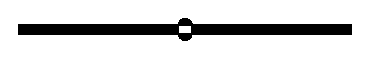
\includegraphics[width=2.5cm]{./images/affine_with_doubled_origin2.eps} / a field $k$.}
    $k$ :: field,
    $X$ :: affine with doubled origin /$k$とする.
    より詳細に,$X$は$X_1=\Spec k[x_1], X_2=\Spec k[x_2]$を
    $U_1=X_1-\{O_1\}, U_2=X_2-\{O_2\}$で貼りあわせたものとする.
    ただし$O_1 \in X_1,O_2 \in X_2$は原点である.
    $X_i, U_i, O_i ~~(i=1,2)$はすべて$X$の部分集合とみなす.
    また$U=X_1 \cap X_2=X-\{O_1, O_2\}$とする.
    明らかに$U=U_1=U_2 \iso \affine^1-\{0\}=\Spec k[x_1, x_1^{-1}]$.
    また$x_1|_U=x_2|_U$.

    \paragraph{Plot.}
    まず,$X$上のinvertible sheaf全体$\Pic X$がどのようなものか調べる.
    これは$\Pic X \iso \Z$となる.
    $n \in \Z$に対応する$\Pic X$の元を$\shL_n$とする.
    次に,generated by global sectionであるようなinvertible sheafを考える.
    これは$\shL_0(=\shO_X)$しかない.
    すると任意の$m>0, n \neq 0$について
    \begin{align*}
        \shL_0 \otimes (\shL_n)^{\otimes m} &= \shL_{mn} \neq \shL_0. \\
        \shL_n \otimes (\shL_0)^{\otimes m} &= \shL_n \hspace{7pt}\neq \shL_0.
    \end{align*}
    なので,どのinvertible sheafもampleでない.

    \paragraph{$X$ :: noetherian integral scheme.}
    $X_1, X_2 \iso \affine^1=\Spec k[x_1]$とreducedがlocalな性質であることから
    $X$ :: noetherian reduced scheme.
    $X$ :: irreducibleも明らかだから,
    $X$ :: noetherian integral scheme.

    \paragraph{$\Pic X \ni \shL=\shL(D)$.}
    $\shL \in \Pic X$を任意にとる.
    $X$ :: integralとProp6.15より,
    $\shL=\shL(D)$となる$D \in \CaCl X$が存在する.
    Prop6.13の証明から$D$がどのような形のものか考えよう.
    Example 6.3.1, Cor 6.16より,$\Pic X_1, \Pic X_2$.
    なので$\shL|_{X_1} \iso \shO_{X_1}, \shL|_{X_2} \iso \shO_{X_1}$となる.
    Prop6.13の証明から,$D$は次のような形をしている.
    \[
        D=\{ \sect{X_1}{f_1}, \sect{X_2}{f_2} \}
        \mwhere
        f_1 \in \Gamma(X_1, \shK_{X_1}^*)=(k(x_1))^*,
        f_2 \in \Gamma(X_2, \shK_{X_2}^*)=(k(x_2))^*.
    \]

    \paragraph{$D \sim \{ \sect{X_1}{x_1^n}, \sect{X_2}{1} \}$.}
    Cartier divisorの定義から,
    $U=X_1 \cap X_2$において$f_1/f_2 \in \Gamma(U, \shO_U^*)$となっている.
    $U \subseteq X_1=\Spec k[x_1]$と考えると,
    $U=\Spec k[x_1]_{x_1}=\Spec k[x_1, x_1^{-1}]$.
    ($U \subseteq X_1$と見れば$U=\Spec k[x_2,x_2^{-1}]$であるが,どちらでも同じである.)
    そして
    \[ \Gamma(U, \shO_U^*)=(k[x_1, x_1^{-1}])^*=\{ \alpha x_1^{n} \mid \alpha \in k^*, n \in \Z \}. \]
    であるから,$f_1/f_2=\alpha x_1^{n} (\iff f_2/f_1=(\alpha x_2^n)^{-1})$と書ける.
    よって
    \[
        D
        =\{ \sect{X_1}{\alpha x_1^n f_2}, \sect{X_2}{f_2} \}
        \mwhere
        f_2 \in \Gamma(X_2, \shK_{X_2}^*)=(k(x_2))^*.
    \]
    再び$X$ :: integralから,$\shK_X$はconstant sheafであり,
    したがって$f_2 \in K=\Gamma(X, \shK_X^*)$となる.
    なので
    $\{ \sect{X_1}{f_2}, \sect{X_2}{f_2} \}$はprincipal.
    加えて$\{ \sect{X_1}{\alpha}, \sect{X_2}{1} \} \in \Gamma(X, \shO_X^*)$なので
    \footnote
    {
        ここの部分はProp6.13cを用いて
        \[
            \shL(\{ \sect{X_1}{\alpha}, \sect{X_2}{1} \})
            =\shO_X
            =\shL(\{ \sect{X_1}{1}, \sect{X_2}{1} \})
        \]
        故に
        $\{ \sect{X_1}{\alpha}, \sect{X_2}{1} \}
            =\{ \sect{X_1}{1}, \sect{X_2}{1} \}$,
        と理解しても良い.

    },
    結局$D \sim \{ \sect{X_1}{x_1^n}, \sect{X_2}{1} \}$.

    \paragraph{$\Pic X \iso \Z$.}
    $n \in \Z$に対し,次のように定める.
    \[ D_n=\{ \sect{X_1}{x_1^n}, \sect{X_2}{1} \},~~~ \shL_n=\shL(D_n). \]
    これは次の写像を定める.
    \begin{defmap}
        {}& \Z& \to& \CaCl X \\
        {}& n& \mapsto& D_n
    \end{defmap}
    明らかに$D_m+D_n=D_{m+n}, \shL_m \otimes \shL_n=\shL_{m+n}$だから,
    これは加法群としての全射準同型.
    最後に,単射であることを見よう.
    $D_n=D_0$ならば,$D_0$同様$D_n$もprincipalである.
    したがって次を満たす$f \in \Gamma(X, \shK_X^*)$が存在する.
    \[
        f|_{X_1}/x_1^n \in \Gamma(X_1, \shO_{X_1}^*)=k^*,~~~
        f|_{X_2}/1 \in \Gamma(X_2, \shO_{X_2}^*)=k^*
    \]
    ここから$f|_{X_1} \in k^*$が得られる.
    よって$(f|_{X_1})/x_1^n \in k^*$と合わせて$n=0$を得る.
    このことは次の段落でも使うので,別に主張として述べておく.

    \begin{Claim}
        $f \in \Gamma(X, \shK_X^*)$とする.
        $f|_{X_2} \in k^*$ならば,$f|_{X_1} \in k^*$.
    \end{Claim}
    \begin{proof}
        $f|_{X_2} \in k^*$から$f|_U \in k^*$が得られる.
        $f|_U=\alpha$としよう.
        $U=\Spec k[x_1]_{x_1} \subset X_1$をみなして考えると,
        $k[x_1]_{x_1}$の元として$(f|_{X_1})|_U=\alpha$となっている.
        なので整数$r \geq 0$が存在し,
        $k[x_1]$の元として$x_1^r(f|_{X_1}-\alpha)=0$.
        しかし$k[x_1]$は整域なので,結局$f|_{X_1}=\alpha \in k^*$.
    \end{proof}
    \begin{proof}
        $k^* \subseteq \shO_{X, O_1}^* \cap \shO_{X, O_2}^*$だから,
        $f_{O_2} \in k^*$より$f_{O_1} \in k^*$.
        他の点における$f$のgermが$k^*$に含まれることは$f|_{X_2} \in k^*$より明らか.
        よって$f \in \Gamma(X, \shO_X^*)=k^*$.
    \end{proof}
    この主張は$X$がnon-separatedであることを暗示している.
%    $R$を$k[x_?]_{(x_?)}$とすると,これは$\shO_{X,O_1}, \shO_{X, O_2}$と同型なDVRである.
%    Ex4.5の用語を使えば「$R$は二つのcenter :: $O_1, O_2$を持つ」と言える.
%    Ex4.5より,これは$X$がnon-separatedであることを意味している.

    \paragraph{Globally Generated Invertible Sheaf on $X$.}
    $n \in \Z$を任意にとり,
    $\{g_i\}_i \subseteq \Gamma(X, \shL_n)$が$\shL_n$のglobal generatorsであるとしよう.
    $\shL_n=\shL(D_n)$だから,
    $\shL_n|_{X_1}$は$x_1^n$でgenerateされ,
    $\shL_n|_{X_2}$は$1$でgenerateされている.
    特に後者から,$\shL_n|_{U}$は$1$でgenerateされている.
    したがってstalkで見れば,次のようになっている.
    \begin{align*}
        \Forall{P \in X_2}
        &\langle \{(g_i)_{P}\}_i \rangle
            \hspace{3.5pt}
            =(\shL_n)_{P}
            \hspace{3.7pt}
                =\shO_{X, P}
                    &&\text{  as  $\shO_{X, P}$-module.} \\
        &\langle \{(g_i)_{O_1}\}_i \rangle_i
            =(\shL_n)_{O_1}
                =(x_1^n)_{O_1} \shO_{X, O_1}
                    &&\text{  as  $\shO_{X, O_1}$-module.}
    \end{align*}
    これらを可換環に翻訳し,
    $g_i$を$g_i|_{X_2}, g_i|_U, g_i|_{X_1}$の順に求めていく.
    $X_2=\Spec k[x_2]$だから,
    $P$に対応する素イデアル$\I{p} \subset k[x_2]$がとれる.
    また,$g_i|_{X_2} \in \Gamma(X_2, \shO_X)=k[x_2]$.
    $\shO_{X,P}=\shO_{X_2, P}=k[x_2]_{\I{p}}$であり,
    したがって$k[x_2]_{\I{p}}$-moduleとして
    $\langle (g_i|_{X_1})_{\I{p}} \rangle=k[x_2]_{\I{p}}$.
    なので,次が成り立つ.
    \[
        \Forall{\I{p} \in \Spec k[x_2]} \Forall{i}
        (g_i|_{X_2})_{\I{p}} \in (k[x_2]_{\I{p}})^*=k[x_2] \setminus \I{p}.
    \]
    よって$g_i|_{X_2} \in (k[x_2])^*=k^*$がわかる.
    前段落に書いた主張から$g_i|_{X_1} \in k^*$.
    $\langle (g_i)_{O_1} \rangle_i=(x_1^n)_{O_1} \shO_{X, O_1}$
    と合わせて$(g_i|_{X_1})/x_1^{n} \in k^*$が得られ,$n=0$となる.
    以上より,$\shL_0$のみがgenerated by global sectionsである.

    \paragraph{Another Proof: Globally Generated Invertible Sheaf on $X$.}
    $n \in \Z$をとり,
    $\{g_i\}_i \in \Gamma(X, \shL_n)$を$\shL_n$のglobal generatorとする.
    $\shL_n|_{X_1}$は$x_1^n$で,$\shL_n|_{X_2}$は$1$で生成されており,
    $X_1, X_2$共にaffine schemeである.
    そのため,次のようになる.
    \begin{align*}
        &\langle \{ g_i|_{X_2} \}_i \rangle
            =\Gamma(X_2, \shL_n|_{X_2})
               =k[x_2]
                    &&\text{  as  $k[x_2]$-module.} \\
        &\langle \{ g_i|_{X_1} \}_i \rangle
            =\Gamma(X_1, \shL_n|_{X_1})
                =x_1^n k[x_1]
                    &&\text{  as  $k[x_1]$-module.}
    \end{align*}
    一行目から,$\{g_i|_{X_2}\} \subseteq (k[x_2])^*=k^*$.
    なので前々段落の主張から,$\{g_i|_{X_1}\} \subseteq k^*$.
    よって$x_1^n \in (k[x_1])^*=k^*$が得られる.

    \paragraph{資料.}
    詰まったところでは次のページを参考にした:
    \url{ https://math.stackexchange.com/questions/70042 }.
          
\section{Ample and Very Ample are Inherted by Tensor Products.} %% Ex7.5 
    $X$ :: noetherian scheme,
    $\shL, \shM$ :: invertible sheaves on $X$
    とする.
    \textbf{``generated by global sections"はgbgsと略す.}
    (d), (e)では更に
    $X$ :: finite type over a noetherian ring $A$,と仮定する.
    (これはThm7.6の仮定である.)

    \begin{Lemma}
        If $\shM, \shM'$ :: gbgs invertible sheaves on $X$,
        then $\shM \otimes_{\shO_X} \shM'$ :: gbgs.
    \end{Lemma}
    \begin{proof}
        $\{m_i\} \subseteq \Gamma(X, \shM), \{m'_j\} \subseteq \Gamma(X, \shM')$を
        それぞれ$\shM, \shM'$のglobal generatorとする.
        定義より,このことは次と同値である:
        任意の点$x \in X$について$\shM_x, \shM'_x$はそれぞれ
        $\{(m_i)_x\}_i, \{(m'_i)_x\}_j$で$\shO_{X,x}$-moduleとして生成される.
        さて,tensor productはleft adjointであることからcolimitと交換する.
        なので$(\shM \otimes_{\shO_X} \shM')_x$は
        $\shM_x \otimes_{\shO_{X,x}} \shM'_x$と同型である.
        明らかにこれは$\{(m_i)_x \otimes (m'_i)_x\}_{i,j}$で生成される
        (Ati-Mac \S2.7)から,$\shM \otimes_{\shO_X} \shM'$ :: gbgs.
        global generatorは$\{m_i \otimes m'_i\}_{i,j}$である.
    \end{proof}

    \subsection{If $\shL$ :: ample and $\shM$ :: gbgs then $\shL \otimes \shM$ :: ample.}
        $\shF$ :: coherent sheaf on $X$とする.
        $\shL$ :: ampleなので,十分大きな$n>0$について
        $\shF \otimes \shL^{\otimes n}$ :: gbgs.
        これに$\otimes \shM^{\otimes n}$を合わせて整理すると,
        補題から$\shF \otimes (\shL \otimes \shM)^{\otimes n}$ :: gbgs.
        よって$\shL \otimes \shM$ :: ample.

    \subsection{If $\shL$ :: ample and $\shM$ :: arbitrary
        then $\shM \otimes \shL^{\otimes n}$ :: ample for some $n>0$.}
        $\shM$ :: coherentなので,十分大きな$n>0$について
        $\shM \otimes \shL^{\otimes n}$ :: gbgs.
        任意の$\shF$ :: coherent sheafに対して十分大きい$r>0$をとると,
        $\shF \otimes \shL^{\otimes rn}$ :: gbgs.
        補題より次もgbgs:
        \[ (\shF \otimes \shL^{\otimes rn}) \otimes (\shM \otimes \shL^{\otimes n})^{\otimes r}. \]
        整理して$\shF \otimes (\shM \otimes \shL^{\otimes 2n})^{\otimes r}$ :: gbgs.
        よって$\shM \otimes \shL^{\otimes 2n}$ :: ample.

    \subsection{If $\shL, \shM$ :: ample then $\shL \otimes \shM$ :: ample.}
        $\shF$ :: cohenrent sheaf on $X$とする.
        十分大きな$l>0$について,$\shF \otimes \shL^{\otimes l}$ :: gbgs.
        このsheafもcoherentなので,十分大きな$m>0$について
        $\shF \otimes \shL^{\otimes l} \otimes \shM^{\otimes m}$ :: gbgs.
        $n=\max(l,m)$とすれば
        $\shF \otimes \shL^{\otimes n} \otimes \shM^{\otimes n}$ :: gbgs.
        整理すれば$\shL \otimes \shM$ :: ampleが得られる.

    \subsection{If $\shL$ :: very ample and $\shM$ :: gbgs then $\shL \otimes \shM$ :: very ample.}
    $\shL, \shM$に対応するmorphismを,
    それぞれ$i: X \to \proj^m_A, j: X \to \proj^n_A$とする.
    Thm7.1bより,$\shL \iso i^* \shO(1), \shM \iso j^* \shO(1)$.
    この時,次の(1)のような$2$重のfiber productを考える.
    ここでの$\proj^N$は$\proj^m, \proj^n$のCartesian product(Ex5.11)であり,
    $N=mn+m+n$である.
    \[
        (1)
        \xymatrix@C=12pt
        {
            {} & X \ar@/^15pt/[rrd]^-{i}\ar@/_15pt/[ddr]_-{j}\ar[rd]^-{\phi}& {} &  {} \\
            {} & {} & \proj^{N}_A \ar[r]^-{p_1}\ar[d]_-{p_2}& \proj^m_A \ar[d] \\
            {} & {} & \proj^n_A \ar[r]& \Spec A
        }
        \hspace{40pt}
        (2)
        \xymatrix@C=12pt@R=40pt
        {
            X \ar[d]_(.3){i}\ar[rrd]^(.25){j}\ar[rr]^-{\phi}&
                {} &
                \proj^m \times \proj^n \ar[lld]_(.3){p_1}\ar[d]^(.3){p_2}\ar[rrr]^-{\psi}&
                {} &
                {} &
                \proj^N \\
            \proj^m \ar[r]& \Spec A &\ar[l] \proj^n & {} & {}
        }
    \]
    (1)の図式にclosed immersion :: $\psi$を加えたのが(2)である.
    (2)の図式で$\omega=\psi \circ \phi$とする.
    $\omega^*\shO_{\proj^N}(1)$を計算すると,次のようになる.
    $\omega^*=\phi^*\psi^*$に注意せよ
    \footnote
        {
            もう少し詳しく述べておこう.
            $X \xrightarrow{f} Y \xrightarrow{g} Z$を考える.
            $f^* g^*$は$g_* f_*=(g \circ f)_*$とadjoint.
            そして$(g \circ f)_*$は$(g \circ f)^*$とadjoint.
            これとadjointの一意性から$f^* g^* \iso (g \circ f)^*$が得られる.
        }.
    \begin{align*}
        {}&     ~\omega^*\shO_{\proj^N}(1) \\
        \iso&   ~\phi^*\shO_{\proj^m \times \proj^n}(1) \\
        \iso&   ~\phi^* (p_1^* \shO_{\proj^m}(1) \otimes_A p_2^* \shO_{\proj^m}(1)) \\
        \iso&   ~\phi^* p_1^* \shO_{\proj^m}(1) \otimes_A \phi^* p_2^* \shO_{\proj^m}(1) \\
        \iso&   ~(p_1 \circ \phi)^* \shO_{\proj^m}(1) \otimes_A (p_2 \circ \phi)^* \shO_{\proj^m}(1) \\
        \iso&   ~i^* \shO_{\proj^m}(1) \otimes_A j^* \shO_{\proj^m}(1) \\
        \iso&   ~\shL \otimes_A \shM
    \end{align*}
    上から順に,
    Ex5.11,
    Ex5.1の解答にある補題,
    図式の可換性を用いている.
    最後に$\omega$がimmersionであることを示そう.
    \begin{Claim}
        $i: X \to \proj^m_A$をimmersionとする.
        次の可換図式において,$\psi \circ \phi: X \to \proj^N_A$はimmersionである.
        \[ 
        \xymatrix@C=12pt@R=40pt
        {
            X \ar[d]_(.3){i}\ar[rrd]^(.25){j}\ar[rr]^-{\phi}&
                {} &
                \proj^m \times \proj^n \ar[lld]_(.3){p_1}\ar[d]^(.3){p_2}\ar[rrr]^-{\psi}&
                {} &
                {} &
                \proj^N \\
            \proj^m \ar[r]& \Spec A &\ar[l] \proj^n & {} & {}
        }
        \]
    \end{Claim}
    \begin{proof}
        次の3つが示せる.
        \begin{enumerate}[label=(\roman*)]
            \item closed immersion :: immersion.
            \item composition of two immersion :: immersion.
            \item immersion :: stable under base cahnge.
        \end{enumerate}
        するとEx4.8の結果がimmersionについて使える.
        まず,図式において,$p_1$はprojective over $A$かつ$A$ :: noetherian ring.
        したがってEx4.9からseparatedである.
        なのでEx4.8eより$\phi$ :: immersion.
        $\psi$ :: immersionとあわせて$\psi \circ \phi$ :: immersion.
        
        上の項目において,(ii)は一般には成立しない.
        しかし$X$ :: noetherian schemeなので,
        immersionはclosed $\circ$ openにもopen $\circ$ closedにも分解でき,
        このことを用いて(ii)が示せる.
        \url{https://stacks.math.columbia.edu/tag/01QV}を参照するとよい.
    \end{proof}

    \subsection{If $\shL$ :: ample then $\shL^{\otimes n}$ :: very ample for sufficiently large all $n>0$.}
    Thm7.6より,ある正整数$l>0$について$\shL^{\otimes l}$ :: very ample.
    また,$\shL$ :: ampleより,
    正整数$m_0>0$が存在し,
    任意の整数$m \geq m_0$について$\shO_X \otimes \shL^{\otimes m}$ :: gbgs.
    したがって,$N=n+m_0$とおけば,(d)より
    \[ (\shO_X \otimes \shL^{\otimes m}) \otimes \shL^{\otimes l}=\shL^{\otimes n} ~~~ (m \geq m_0, n \geq N) \]
    はvery ampleである.

\section{The Riemann-Roch Problem.} %% Ex7.6 
    $k$ :: algebraically closed field,
    $X$ :: nonsingular projective variety over $k$,
    $D$ :: divisor on $X$
    とする.
    (したがって$|D|$ :: linear systemが考えられる.)
    この時,$n$の関数$\dim_k |nD|$を考える.
    $\shL$を$D$に対応するinvertible sheafとすると,
    Prop7.7より,これは$\dim_k \Gamma(X, \shL^n)-1$とも書ける.

    Ex2.14とCor5.16を合わせると,
    $X=\Proj k[x_0, \dots, x_d]/I$なる$I$ :: homogeneous idealが
    存在することが分かる.
    そこで$S=k[x_0, \dots, x_d], T=S/I$としておく.
    また$\phi: S \to T=S/I$を標準的全射としておく.

    \subsection{$D$ :: very ample $\implies \Forall{n \gg 0} \dim_k |nD|=P_X(n)-1$.}
    今,$\shL$ :: very ampleだから,
    $i^* \shO_{\proj^d}(1) \iso \shL$となる
    closed immersion $i: X \to \proj^d_k$が存在する.
    (closedであることはRemark5.16.1と同様.)
    Ex6.8a($i^*$と$\otimes$が分配的であること)とProp5.12(の証明)から次が分かる.
    \[
        \shL^{\otimes n}
        =(i^* \shO_{\proj^d}(1))^{\otimes n}
        \iso i^* ((\shO_{\proj^d}(1))^{\otimes n})
        \iso i^* (S(n) \sidetilde)
        \iso (S(n) \otimes T)\sidetilde.
    \]
    $\phi$が次数を保つこと(したがって$\phi(S(n))=T(n)$)から,
    $S(n) \otimes T \iso T(n)$.
    Ex5.9bより,十分大きい全ての$n$について$T_n \iso \Gamma(X, (T(n))\sidetilde)$となる.
    よって,
    $P_X$を$X$のHilbert polynomialとすると,
    十分大きい全ての$n$について$P_X(n)=\dim_k \Gamma(X, \shL^{\otimes n})$.

    \subsection{If $D$ is torsion element of order $r$,
        then $\dim_k |nD|=0$ if $r \divible n$ \& $=-1$ otherwise}

    orderの定義から,$nD=0 \iff n \bmod r=0$であることに注意する.
    次を示す.
    \[
        \dim_k |nD|=
        \begin{cases}{}
            0   & n \bmod r=0 \\
            -1  & n \bmod r \neq 0
        \end{cases}
    \]

    \paragraph{$n \bmod r=0 \implies \dim_k |nD|=0$.}
    $n \bmod r=0$の時,$nD=0$,$\shL^{\otimes n}=\shO_X$.
    今,$X$ :: integral \& proper \& finite type scheme over algebraically closed subset.
    なのでEx4.5dより,$\Gamma(X, \shO_X)=k$.
    よって$\dim_k |nD|=\dim_k \Gamma(X, \shO_X)-1=0$.

    \paragraph{$n \bmod r \neq 0 \implies |nD|=\emptyset \implies \dim_k |nD|=-1$.}
    $n \bmod r \neq 0$の時,$|nD|=\emptyset$を示す.
    $E=\{\sect{U_i}{f_i}\}_i \in |nD|$がとれるとして矛盾を導くことにする.
    $E$ :: effectiveかつ$E \sim nD \not \sim 0$なので,
    $f_i \in \Gamma(U_i, \shO_{U_i})$は単元でない.
    したがって$f_i^r$も単元でない
    \footnote
    {
        $f_i$は単元でないから,$\Gamma(U_i, \shO_{U_i})$の真のイデアルに属す.
        そして$f_i^r$もこのイデアルに属し,
        したがって$f_i^r$は単元でない.
    }.
    いずれの$i$についても同様なので,
    $rE$はprincipalでない($rE \not \sim 0$).
    一方,$E \sim nD, rD=0$だから$rE \sim rnD \sim 0$.

\section{Some Rational Surfaces.} %% Ex7.7 

\section{Sections of $\pi: X \to \pbundle(\shE)$
    $\leftrightarrow$ Quotient Invertible Sheaves of $\shE$.} %% Ex7.8 

    $X$ :: noetherian scheme,
    $\shE$ :: coherent locally free sheaf on $X$とする.
    Prop7.12において$Y=X, g=\id[X]$とすると,
    以下の図式を成立させる$\sigma: X \to \pbundle(\shE)$と
    quotient invertible sheaf of $\shE $:: $\shE \to \shL \to 0$が
    \footnote
    {
        $\shE \to \shL \to 0$だけで$\shL$と全射 :: $\shE \to \shL$の組を意味する.
        $g^*\shE=\shE$に注意.
    }
    対応することがわかる.
    \[
        \xymatrix
        {
            X \ar[r]^-{\sigma}\ar[d]_-{\id[X]}& \pbundle(\shE) \ar[ld]^-{\pi} \\
            X
        }
    \]
    明らかに$\sigma$は$\pi$のsectionである.
    
    \begin{Remark}
        $\shL$ :: invertible sheaf on $X$とする.
        一般に次が成り立つ.
        \[ \Hom(\shL, \shO_X)=\Gamma(X, \shHom(\shL, \shO_X))=\Gamma(X, \shL^{-1}).\]
        $X=\Proj A[x_0,\dots,x_n], \shL=\shO(n) ~(n>0)$の時は,
        Prop5.13と合わせて$\Hom(\shL, \shO_X)=0$が得られる.
        $X$がEx5.14の条件を満たすときについても同じことが言える.
    \end{Remark}

\section{$\Pic \pbundle(\shE) \iso \Pic X \oplus \Z$.} %% Ex7.9 
    $X$ :: \textbf{connected} regular noetherian scheme,
    $\shE$ :: locally free coherent sheaf of rank $\geq 2$ on $X$とする.
    $r=\rank \shE (\geq 2)$とおく.
    また$P=\pbundle(\shE)$としておく.

    \subsection{$\Pic \pbundle(\shE) \iso \Pic X \oplus \Z$.}
    これはEx6.1 ($\Pic \proj_X^n \iso \Pic X \oplus \Z$) のrelatively versionである.

    \subsubsection{方針.}
    次の写像が同型写像であることを示す.
    \begin{defmap}
        \phi:& \Pic X \oplus \Z& \to& \Pic \pbundle(\shE) \\
        {}& \shL \oplus n& \mapsto& \pi^* \shL \otimes \shO_P(n)
    \end{defmap}
    $\pi^*$が準同型である(Ex6.8a)から,$\phi$が準同型であることは明らか.
    $\phi$ :: surjが難しい部分である.
    これは3つの部分に分けられる.
    $U$ :: irreducible affine open subset in $X$,
    $V=\pi^{-1}(U) (\iso \proj_A^{r-1})$とする.
    \begin{enumerate}[label=(\alph*)]
        \item Ex6.1の結果を$\Pic V$の場合に翻訳する.
        \item $\shL|_V$が$\shO_V(n_U)$と書けるとき$n_U$は$U$に依存しないことを示す.
        \item $\shL|_V$が$\pi^* \shM_U ~(\shM_U \in \Pic U)$と書けるとき$\shL$は$\pi^* \shM$と書けることを示す.
    \end{enumerate}

    \subsubsection{$\phi$ :: inj.}
    $\phi(\shL \oplus n)=\pi^* \shL \otimes \shO_P(n) \iso \shO_P$となる
    $\shL \oplus n \in \Pic X \oplus \Z$が存在したとする.
    両辺に$\pi_*$を作用させてEx5.1d (Projective formula), Prop7.11aを用いると次のよう.
    \[ \shL \otimes \Sym^n(\shE) \iso \shO_X. \]
    両辺の$\rank$を計算すると$\binom{r+n-1}{r-1}=1$ (Ex5.18a).
    よって$r-1=0 \mor r+n-1$となり,$r \geq 2$より$n=0$が得られる.
    さらに$n=0$から$\shL \otimes \Sym^n(\shE) \iso \shL\iso \shO_X$.
    まとめて,$\phi$ :: inj.

    \subsubsection{$\phi$ :: surj.}
    $\pbundle(\shE)$上の任意のinvertible sheafが
    $\pi^* \shL \otimes \shO_P(n)$の様に書けることを示さなくてはならない.
    まず,localにはそれが出来ることを示す.

    $U$ :: irreducible affine open subset in $X$, 
    $V=\pi^{-1}(U) (\iso \proj_A^{r-1})$とする.
    $X$ :: regular noetherian schemeだから,
    Prop4.1と合わせて$U$ :: ($*$) (p.130).
    またCor6.16が成り立つ.
    \begin{Claim}
        $X$を,Cor6.16が成立するものとする(特に$X$ :: integral).
        $Y=\proj^n_X(=\proj^n_{\Z} \times X)$とし,
        また$\pi: Y \to X$をprojection of fiber productとする.
        $Z$ :: prime divisor in $X$をとる.
        Cor6.16の同型写像$\Cl X \isomap \Pic X$によって,
        $\shL \in \Pic X$が$Z$に対応するならば,
        $\pi^* \shL \in \Pic Y$は
        $\pi^* Z=\pi^{-1}(Z)$ (cf. Prop6.6)に対応する.
    \end{Claim}
    \begin{proof}
        U.G\"orts, T.Wedhorn ``Algebraic Geometry I" p.312にある
        ``(11.16) Inverse image of divisors."を参照した.

        準備として,
        $y \in Y$について$\pi^{\#}_{\pi(y)}: \shO_{X, \pi(y)} \to \shO_{Y, y}$を調べよう.
        $\pi(y) \in V=\Spec A, y \in U=\Spec A[x_0,\dots,x_n]_{(f)} (\subset \pi^{-1}(V))$とする.
        ただし$f \in A[x_0,\dots,x_n]$は正次数をもつ斉次元である.
        今,projection :: $\pi|_U$は
        包含写像$A \inclmap A[x_0,\dots,x_n]_{(f)}$から誘導されている
        \footnote
        {
            より正確には$A \to A \otimes \Z[x_0,\dots,x_n]_{(f)};~ a \mapsto a \otimes 1$から誘導されている.
            しかし$A \otimes \Z[x_0,\dots,x_n]_{(f)} \iso A[x_0,\dots,x_n]_{(f)};~ a \otimes b \mapsto ab$を通せば
            これは単なる包含写像である.
        }.
        なので$y, \pi(y)$に対応する素イデアルを
        それぞれ$\I{p}, \I{q}$とすると$\I{q}=\I{p} \cap A$が成り立つ.
        また$\pi^{\#}_{\pi(y)}=(\pi|_U)^{\#}_{\pi(y)}$だから,
        $\pi^{\#}_{\pi(y)}$も包含写像である.

        ここで,$l \geq 0$について$\I{q}^{l}=\I{p}^{l} \cap A$が成り立つことに注意する.
        このことから,$a \in A$について
        \[ \pi^{\#}_{\pi(y)}(a)=a \in \I{p}^{l} \iff a \in \I{q}^{l}. \]
        一般に,DVR :: $(R, \I{m})$のvaluation :: $v_R$は
        $r \in R$について次を満たす.
        \[ v_R(r)=\sup \left\{ l \geq 0 \,\middle|\, r \in \I{m}^l \right\}. \]
        したがって$\shO_{X, \pi(y)}, \shO_{Y, y}$が共にDVRである時,
        $\pi^{\#}_{\pi(y)}$はvaluationを保つ.
        \[
            v_y \left( \pi^{\#}_{\pi(y)}(*) \right)
            =\sup \left\{ l \geq 0 \,\middle|\, \pi^{\#}_{\pi(y)}(*) \in (\I{m}_{Y,y})^l \right\}
            =\sup \left\{ l \geq 0 \,\middle|\, * \in (\I{m}_{X,\pi(y)})^l \right\}
            =v_{\pi(y)}(*)
        \]

        いよいよinvertible sheafとdivisorの関係を調べていく.
        $Z$のgeneric pointを$\zeta$とし,
        $Z$に対応するCartier divisorを
        $D=\{\sect{U_i}{f_i}\}_i \in \CaCl X$とする.
        $x \in X$をcodimension oneの点だとすると,
        Prop6.11の証明にある$D$の構成方法から,
        次が成り立つ.
        \[
            v_x((f_i)_x)=
            \begin{cases}{}
                1   &   x=\zeta \\
                0   &   x \neq \zeta.
            \end{cases}
        \]
        $v_x$はDVR :: $\shO_{X,x}$のvaluationである.
        ($X$について仮定から($*$)が成立していることに注意.)
        $i$は$x \in U_i$であるものならばどれでも良い.
        また,$Z$ :: effectiveから,$D$ :: effective (Remark 6.17.1).
        すなわち,各$i$について$f_i \in \Gamma(U_i, \shO_{U_i})$.

        $\pi^* \shL$の$y \in Y$でのstalkを見る.
        $\pi(y) \in U_i \subseteq X$なる$i$を一つとって固定すると,次が成り立つ.
        \[
            (\pi^* \shL)_y
            \iso \shL_{\pi(y)} \otimes_{\shO_{X, \pi(y)}} \shO_{Y, y}
            =
            \left[ (f_i^{-1})_{\pi(y)} \otimes 1_{\shO_{Y, y}} \right]
            \shO_{X, \pi(y)} \otimes_{\shO_{X, \pi(y)}}\shO_{Y, y}.
        \]
        最左の$\iso$はleft adjoint preserves colimits (LAPC)を用いて示すことが出来る.
        今,$\pi^{\dsharp}_{\pi(y)}: \shO_{X, \pi(y)} \to \shO_{Y, y}$を用いて
        $\shO_{Y, y}$を$\shO_{X, \pi(y)}$-module (submodule of $\shK_{Y,y}$)とみなしている.
        したがって更に計算が出来て次が得られる.
        \[ (\pi^* \shL)_y \iso [\pi^{\#}_{\pi(y)}((f_i)_{\pi(y)})]^{-1}\shO_{Y, y}. \]
        こうして,$\pi^*\shL$に対応するCartier divisorのgermが分かった.

        点$y \in Y, \pi(y) \in X$を共にcodimension oneの点だとする.
        $i$を$\pi(y) \in U_i$なるものとしてとる.
        この時,$X$については仮定から,$Y$についてはEx6.1から($*$)が成立する.
        したがって$v_y(\pi^{\#}_{\pi(y)}((f_i)_{\pi(y)}))$の値が考えられる.
        上述した$v_y \circ \pi^{\#}_{\pi(y)}=v_{\pi(y)}$より,これは次の通り.
        \[
            v_y \left(\pi^{\#}_{\pi(y)}((f_i)_{\pi(y)})\right)=
            v_{\pi(y)}((f_i)_{\pi(y)})=
            \begin{cases}{}
                1 & \pi(y)=\zeta \\
                0 & \pi(y) \neq \zeta.
            \end{cases}
        \]
        よって,
        点$\eta \in Y$を$\pi(\eta)=\zeta$を満たすcodimension oneの点だとすれば,
        $\pi^*\shL$は$\cl_{Y}(\{\eta\})$に対応する.
        計算すると,$\cl_{Y}(\{\eta\})=\pi^{-1}(Z)=\pi^*Z$.
    \end{proof}

    \begin{Cor}
        $D$ :: Weil divisor $U$をとり,
        $\shL \in \Pic U$が$D$に対応するinvertible sheafだとする.
        $\pi^* D$(Prop6.6)に対応するinvertible sheafは$\pi^* \shL$である.
    \end{Cor}

    irreducible \& affine open subset of $X$ :: $U$であって,
    かつ$\shE|_U \iso \shO_U^{\oplus r}$となるようなものからなる
    open coverを$\coverU$とする.
    $X$ :: noetherian schemeから$\coverU$ :: finite cover.

    $U \in \coverU$をとり,$V=\pi^{-1}(U) (\iso \proj^{r-1}_{\Z} \times U)$とする.
    Cor6.16から$\Cl U \iso \Pic U$.
    Ex6.1と上の主張を合わせて,
    $\pbundle(\shE)$上の任意のinvertible sheafは,
    localには(すなわち,$V$に制限すれば)
    $(\pi|_V)^* \shL_U \otimes \shO_V(n_U)$と書ける.
    Cor6.16の証明にあるとおり,
    hyperplane (prime divisor)はtwisted sheafに対応することに注意.

    $\shM \in \Pic P$をとる.
    上での議論から,上のような各$U, V$について
    $\shM|_V \iso (\pi|_V)^* \shL_U \otimes \shO_V(n_U)$.
    任意の$U \in \coverU$で$n_U$が等しいことを示そう.
    適当な$U \in \coverU$について,$n_{U}<0$ならば$\shM$の代わりに$\shM^{-1}$を考える.
    こうすれば,少なくともひとつの$U$について$n_{U} \geq 0$となる.
    projective formulaを用いて以下の計算を行う.
    \begin{align*}
        {}&     (\pi_*\shM)|_{U} \\
        \iso&   (\pi|_V)_* (\shM|_V) \\
        \iso&   \shL_U \otimes (\pi|_V)_* \shO_V(n_U) \\
        \iso&   \shL_U \otimes \Sym^{n_{U}}(\shE)|_U
    \end{align*}
    最後にProp7.11aを用いた.
    $n_U \geq 0$だから,
    この$X$上のlocally free sheafのrankは,$\binom{n_U+r-1}{r-1}$.
    $X$ :: connectedより,$\pi_* \shM$のrankは$U \in \coverU$に依らない.
    すなわち,任意の$U, U' \in \coverU$について
    \[ \binom{n_U+r-1}{r-1}=\binom{n_{U'}+r-1}{r-1} \]
    となる.
    ここから直ちに$n_U=n_{U'}$が得られる.
    この値を$n (=n_U)$としておこう.


    $\shL=\pi_*(\shM \otimes \shO_P(-n))$とおく.
    すると$\shL|_U=\shL_U$が得られる.
    \begin{align*}
        {}&     \shL|_U \\
        \iso&   (\pi|_V)_* (\shM \otimes \shO_P(-n))|_V \\
        \iso&   (\pi|_V)_* (\shM|_V \otimes \shO_V(-n)) \\
        \iso&   (\pi|_V)_* (\pi|_V)^*\shL_U \\
        \iso&   \shL_U
    \end{align*}
    最後にprojective formulaを用いた.
    こうして各$U \in \coverU, V=\pi^{-1}(U)$について
    $\shM|_V \iso (\pi^* \shL \otimes \shO_P(n))|_V$となる.

    あとは$\shM \iso \pi^* \shL \otimes \shO_P(n)$を示せば良い.
    これは次のように示せる.
    $\id[\shL]: \shL \to \pi_*(\shM \otimes \shO_P(-n))$を考える.
    これをadjoint pair :: $\pi^* \dashv \pi_*$を使って写す.
    \[ \pi^* \shL \to \shM \otimes \shO_P(-n). \]
    additive categoryにおけるadjoint functorについての一般論から,
    これは再び同型写像である.
    tensor productは全射性を保つから,
    $\pi^* \shL \otimes \shO_P(n) \to \shM$は全射.
    Ex7.1より,これは同型である.

    \begin{Remark}
        $X$のconnected componentが丁度$g$個ある場合には
        $\Pic \pbundle(\shE) \iso \Pic X \oplus \Z^{\oplus g}$となる.
        具体的に,各connected componentを$C_1,\dots,C_g$とすると,
        $\Pic \pbundle(\shE)$のconnected componentは
        $\pi^{-1}(C_1), \dots, \pi^{-1}(C_g)$.
        そこで$\iota_i: \pi^{-1}(C_i) \hookrightarrow \pbundle(\shE)$を
        包含射とすると同型写像は次のように成る.
        \begin{defmap}
            {}& \Pic X \oplus \Z^{\oplus g}& \to& \Pic \pbundle(\shE) \\
            {}& (\shL, n_1,\dots,n_g)& \mapsto& \pi^* \shL \otimes \left( \bigoplus_{i} (\iota_i)_*(\iota_i)^*\shO_P(n_i) \right)
        \end{defmap}
        証明は$X$の各connected componentごとに上で示したことを用いれば良い.
    \end{Remark}

    \subsection{$\pbundle(\shE) \iso \pbundle(\shE') \iff
        \Exists{\shL \in \Pic X} \shE'=\shE \otimes \shL$.}
    $\shE'$ :: locally free coherent sheaf on $X$とする.
%    ($\rank \shE' \geq 2$という条件はついていない.)
    名前を次のように付ける:
    $P=\pbundle(\shE), \pi: P \to X, P'=\pbundle(\shE'), \pi': P' \to X$.

    \paragraph{$\implies$.}
    $\phi: P' \isomap P$をとる.
    \[
        \xymatrix
        {
            P' \ar@<2pt>[rr]^-{\phi}\ar[rd]_-{\pi'}& {} &\ar@<2pt>[ll]^-{\phi^{-1}} P \ar[ld]^-{\pi} \\
            {} & X & {}
        }
    \]
    $\shO_{P'}(1) \in \Pic P \iso \Pic X \oplus \Z$なので,
    \[ \phi^* \shO_{P'}(1) \iso \shO_P(1) \otimes \pi^* \shL ~~~(\shL \in \Pic X). \]
    左辺は$\Pic P'$の,右辺は$\Pic P$の生成元である.
    (なので$\shO_P(1)$が右辺に現れる.)
    両辺に$\pi_*$を作用させてEx5.1d (Projective formula), Prop7.11aを用いると次のよう.
    \[ \pi_*\phi^* \shO_{P'}(1) \iso \shE \otimes \shL. \]
    あとは$\pi_* \phi^* \iso \pi'_*$を示せば,
    Prop7.11aから主張が得られる.
    $\phi$が同型写像であることに注意して計算する.
    \begin{align*}
        {}&     \Hom(-, \pi_* \phi^* -) \\
        \iso&   \Hom(\pi^* -, \phi^* -) \\
        \iso&   \Hom((\phi^{-1})^*\pi^* -, (\phi^{-1})^*\phi^* -) \\
        \iso&   \Hom(\pi'^* -, -) \\
        \iso&   \Hom(-, \pi'_* -)
    \end{align*}
    よってYoneda principalから$\pi_* \phi^* \iso \pi'_*$.

    \paragraph{$\impliedby$.}
    次を示すと,Lemma7.9から$\pbundle(\shE) \iso \pbundle(\shE')$が得られる.
    \[ \Sym^d(\shE \otimes \shL) \iso \Sym^d(\shE) \otimes \shL^{\otimes d}. \]
    両辺がpresheafとして同型であること,
    すなわち次が成り立つことを示す.
    $U$を$X$の任意の開集合とし,
    $A=\Gamma(U, \shO_X), E=\Gamma(U, \shE) \iso A^{\oplus r}, L=\Gamma(U, \shL)$とする.
    \[ \Sym^d(E \otimes L) \iso \Sym^d(E) \otimes L^{\otimes d}. \]
    $\Sym^d(E \otimes L)$の元をとる.
    これは$E$の元$e_1,\dots,e_d$と$L$の元$l_1,\dots,l_d$を用いて次のように表せる.
    \[ (e_1 \otimes l_1) \otimes \cdots \otimes (e_d \otimes l_d). \]
    また$\Sym^d(E) \otimes L^{\otimes d}$の元は次のよう.
    \[ (e_1 \otimes \cdots \otimes e_d) \otimes (l_1 \otimes \cdots \otimes l_d). \]
    これらが互いに書き換えられることは明らか.
    よって所望の同型が得られる.

\section{$\proj^n$-Bundles Over a Scheme.} %% Ex7.10 

\section{Different Sheaves of Ideals can Give Rise to Isomorphic Blow Up Schemes.} %% Ex7.11 

\section{ } %% Ex7.12 

\section{* A Complete Nonprojective Variety.} %% Ex7.13 

\section{Very ample invertible sheaf on $\gProj$.} %% Ex7.14 
    \begin{Thm}
        Let $S$ be a scheme, and let $X$ be a scheme over $S$.
        If $\shL$ is an invertible sheaf on $X$,
        and if $s_0, \dots ,s_n \in \Gamma(X, \shL)$ are global sections which generate $\shL$,
        then there exists a unique $S$-morphisn1 $\phi:X \to \proj^n_A$ such that 
        $\shL \iso \phi^*(\shO_X(1))$ and $s_i = \phi^*(x_i)$ under this isomorphism.
    \end{Thm}
    \begin{proof}
        この定理はThm7.1bの拡張である.
        前提より,$f: X \to S$がある.
        まず$V=\Spec A \subseteq S$をとり,$U=f^{-1}(V)$としよう.
        すると$f|_U: U \to \Spec A$なる射が出来る.
        そしてThm7.1の証明と同じことを$U$と$\Spec A$に行う.
        ただし,$X_i$の代わりに使うのは$U \cap X_i$である.
        $V$を動かしていけば,$U \cap X_i$で$X$を覆うことができる.
        そして出来上がる大量の射 :: $U \cap X_i \to \Spec A[x_0,\dots,x_n]_{(x_0)}$を
        貼り合わせられることは明らか.
    \end{proof}

    \begin{Thm}
        Let $X$ be a quasi-compact and finite type scheme over a scheme $S$,
        and let $\shL$ be an invertible sheaf on $X$.
        Then $\shL$ is ample if and only if 
        $\shL^{\otimes m}$ is very ample over $S$ for some $m>0$.
    \end{Thm}
    \begin{Remark}
        この定理はThm7.6の拡張である.
        他にこの定理の拡張は様々に述べられているが,
        最も拡張して述べているのはこれであろう:
        $X$ is locally of finite type over $S$
        \footnote{ \url{https://stacks.math.columbia.edu/tag/01VS} }.
        ただし,脚注で示したページにある証明では,
        EGAでのimmersionの定義を用いている.
        また証明には``we can find finitely many such elements"という文があるが,
        この文が成り立つためには$X$ :: quasi-compactが必要である.
        $X$ :: quasi-compactを加えると,
        EGAでのimmersionの定義と教科書でのimmersionの定義が一致する.
        また``$X$ is locally of finite type over $S$"は
        ``$X$ is of finite type over $S$"になる.
        なのでこの命題の仮定は,弱めてもこの命題のように成る.
    \end{Remark}
    \begin{proof}
        まず,$U=\Spec A \subseteq S$をとる.
        そして$f^{-1}(U)$に含まれるaffine open subset :: $V$をとる.
        $X-V$についてp.154最下からp.155最上までの議論を行うと,
        適当な$s \in \Gamma(X, \shL^{\otimes n_s})$について
        $X_s$ :: affine open subset of $X$となる.
        $X_s \subset V \subset f^{-1}(U)$かつ$X_s$ :: affineなので,
        Ex3.3cより$\Gamma(X_s, \shO_X)$ :: finitely generated $A$-algebra.
        $U, s$を動かせば$X$が$X_s$で被覆できる.
        $X$ :: quasi-compactなので,$U, s$は有限個で事足りる.
        $U_i=\Spec A_i$と$s_{ij} \in \Gamma(X, \shL^{\otimes n})$を使うことにしよう.
        $X$ :: quasi-compactを加えると,
        ただし$n=\max_{ij} n_{s_{ij}}$.
        また$X_{ij}=X_{s_{ij}}$とする.
        後の議論はp.155の``Now for each $i$, let $B_i=$..."と全く同じ.
        $A$の代わりに$A_i$を,
        $B_i$の代わりに$B_{ij}=\Gamma(X_{ij}, \shO_X)$を用いる.
        そして$B_{ij}$の$A_i$-algebraとしてのgeneratorを$b_{ijk}$とし,
        これをLemma5.14を用いて拡張して$c_{ijk}$とする.
        $\{ s_{ij}^n \},\{ c_{ijk} \}$は,全て合わせて$N+1$個あるとしよう.
        これらのglobal sectionsを元に,
        上の定理(Thm7.1bの一般化)から$X \to \proj^N_S$の射を得る.
        \[
        \xymatrix
        {
            X \ar[d]_-{f}\ar[r]^-{\phi}& \proj^N_S \ar[ld]^-{\pi'}\\
            S & {}
        }
        \]
        $i,j$を適当にとり,
        $U=U_i \subseteq S, V=\bigcup_j X_{ij}=f^{-1}(U) \subseteq X$とする.
        そこで次の図式を考える.
        \[
        \xymatrix
        {
            V \ar[d]_-{f|_V}\ar[r]^-{\phi|_V}& \proj^N_U \ar[ld]^-{\pi'|_{\proj^N_U}}\\
            U & {}
        }
        \]
        Thm7.6の証明と同様に$\phi|_V$ :: immersion.
        immersionはlocalな性質だから,$\phi$ :: immersion.
    \end{proof}

    \subsection{Example: $\shO_{\pbundle(\shE)}(1)$ is not very ample relative to $X$.}
    $k$ :: field, $X=\proj^1_k, r-1>0, \shE=(\shO_X(-1))^{\oplus r}$とする.
    また$P=\pbundle(\shE)$としておく.

    もし$\shO_P(1)$がvery ampleならば,上のThmから,これはampleでもある.
    したがって十分大きい全ての$n>0$について
    $\shO_P(n)(=\shO_P(1)^{\otimes n})$ :: generated by global sections (以降はgbgsと略す)
    \footnote
    {
        ample sheafの定義において,$\shF=\shO_P$とすると
        $\shF \otimes (\shO_P(1))^{\otimes n}=\shO_P(n)$ :: gbgs.
    }
    .
    しかし次が成り立つ.
    \begin{Claim}
        \[ \Forall{n>0} \Gamma(P, \shO_P(n))=0. \]
    \end{Claim}
    一方,$\shO_P(n)$はinvertible sheafだから$\shO_P(n) \neq 0$.
    したがって$\shO_P(n)$はgbgsでなく,$\shO_P(1)$はvery ampleでない.
    \begin{proof}
        $n>0$を任意にとる.
        $\rank \shE=r \geq 2$であるから,Prop7.11aより次のように成る.
        \[ \Gamma(P, \shO_P(n))=\Gamma(X, \pi_*\shO_P(n))=\Gamma(X, \Sym^n(\shE)). \]
        $\Sym^n(\shE)$の代わりに$T^n(\shE)=\shE^{\otimes n}$を考える.
        \[
            \Gamma(X, \shE^{\otimes n})
            =\Gamma(X, [(\shO_X(-1))^{\oplus r}]^{\otimes n})
            =\Gamma(X, (\shO_X(-n))^{\oplus r}).
        \]
        Ex1.9にあるdirect sumの定義から,
        これは$\Gamma(X, \shO_X(-n))^{\oplus r}$に等しい.
        そしてProp5.13から,これは$\Gamma(X, \shO_X(-n))^{\oplus r}=0$.

        $\Gamma(X, \Sym^n(\shE))$の定義の仕方から,
        $\Gamma(X, T^n(\shE))=0$は$\Gamma(X, \Sym^n(\shE))=0$を意味する.
        よって$\Gamma(P, \shO_P(n))=0$.
    \end{proof}

    \begin{Remark}
        very ampleの定義から$\shO_X(1)$ :: very ample on $X$ relative to $\Spec k$.
        Thmから$\shO_X(1)$ :: ample.
        これらとProp7.10から,十分大きい全ての$n \gg 0$について,
        $\shO_P(1) \otimes \pi^* \shO_X(n)$ :: very ample.
        Prop7.11aから
        $\pi_*(\shO_P(1) \otimes \pi^* \shO_X(n))=\shE(n)$であることも留意せよ.
    \end{Remark}

    \subsection{$\Forall{n \gg 0} \shO_{\pbundle(\shE)}(1) \otimes \pi^* \shL^n$ :: very ample.}
    以下のように設定する.
    \begin{itemize}
        \item $X$ :: noetherian scheme
            \footnote{ 教科書では明記されていないが($\dagger$)の一部である.},
        \item $Y$ :: scheme,
        \item $\shL$ :: ample invertible sheaf on $X$,
        \item $\shJ$ :: sheaf of graded $\shO_X$-algebra satisfying ($\dagger$),
        \item $f: X \to Y$ :: morphism of finite type.
    \end{itemize}
    また$P=\gProj \shJ$とし,$\pi: P \to X$をprojectionとする.
    \[
        \xymatrix
        {
            P \ar[r]^-{\pi}& X \ar[r]^-{f}& Y
        }
    \]
    ``very ample invertible sheaf on $P$ relative to $Y$"を[$P/Y$]と書くことにする.

    $\shL$ :: ample on $X$が存在するので,
    Prop7.10より,
    $\shO_P(1) \otimes \pi^* \shL^{\otimes m}$ :: [$P/X$].
    またThmより十分大きい$n>0$について$\shL^{\otimes n} :: [X/Y]$.
    このこととEx5.12bより以下は$[P/Y]$.
    \[
        (\shO_P(1) \otimes \pi^* \shL^{\otimes m}) \otimes \pi^*(\shL^{\otimes n})
        =\shO_P(1) \otimes \pi^* \shL^{\otimes m+n}
    \]
\end{document}
